\newpage
\section{Task 4: Advanced Entity-Relationship modelling}

The pizza store from Task 3 now requires you to update and expand the previous database you designed for them, in order to record some additional information.

\subsection{Assumptions}

\begin{itemize}
\item A staff member may be a supervisor to many staff members
	\begin{itemize}
	\item A staff member may only have one supervisor
	\item Some staff may not have a supervisor
	\end{itemize}
\item A staff member may not deliver any pizzas
\item A PizzaType must include one PizzaRange selection
	\begin{itemize}
	\item It is possible that a PizzaRange may never be selected for a PizzaOrder
	\end{itemize}
\end{itemize}

\subsection{Logical E-R diagram}

\begin{figure}[H]
\centering
\caption{Pizza Store Advanced Logical E-R Diagram}
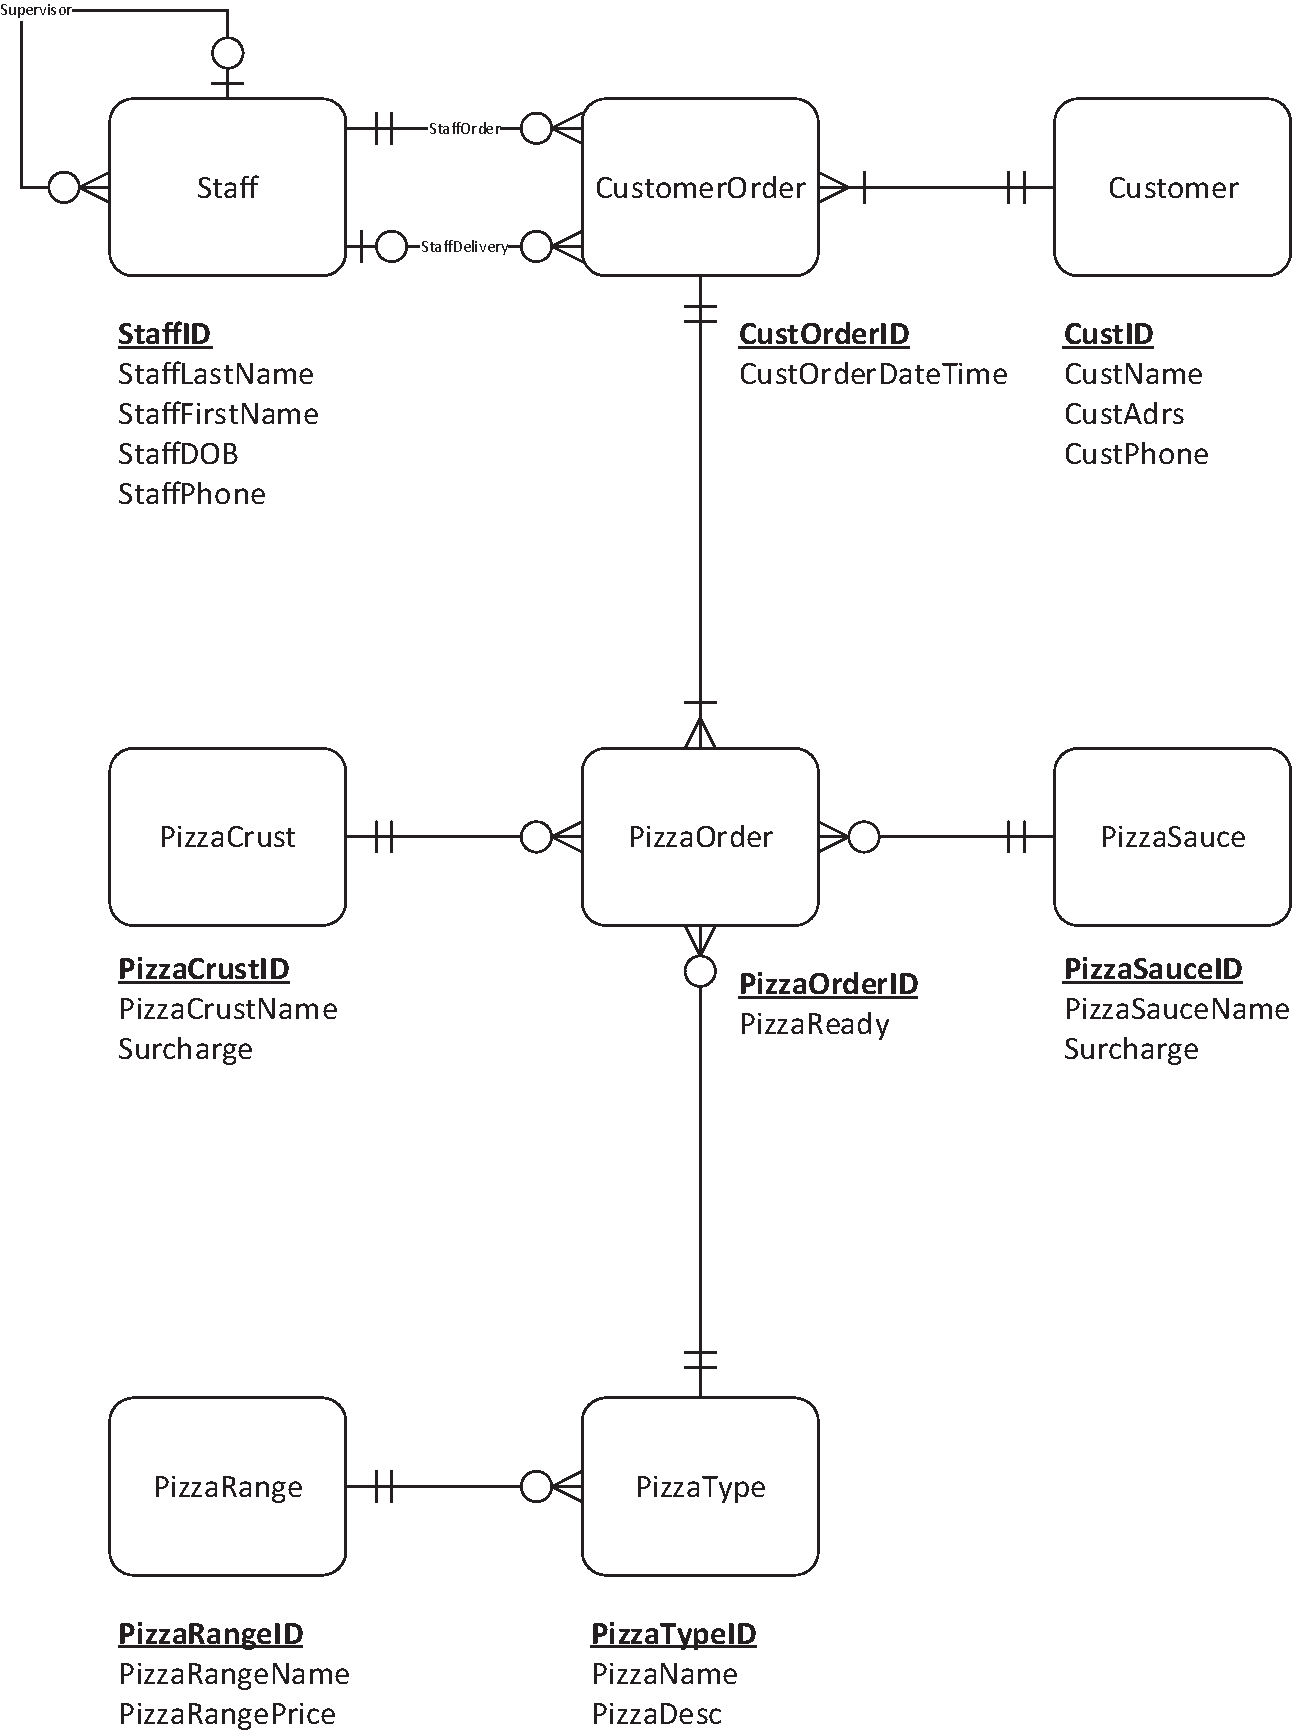
\includegraphics[scale=0.5]{./img/CSG1207_A1_PONCE_TASK_4_ADVLER_PIZZA.pdf}
\end{figure}

\subsection{Physical E-R diagram}

\begin{figure}[H]
\centering
\caption{Pizza Store Advanced Physical E-R Diagram}
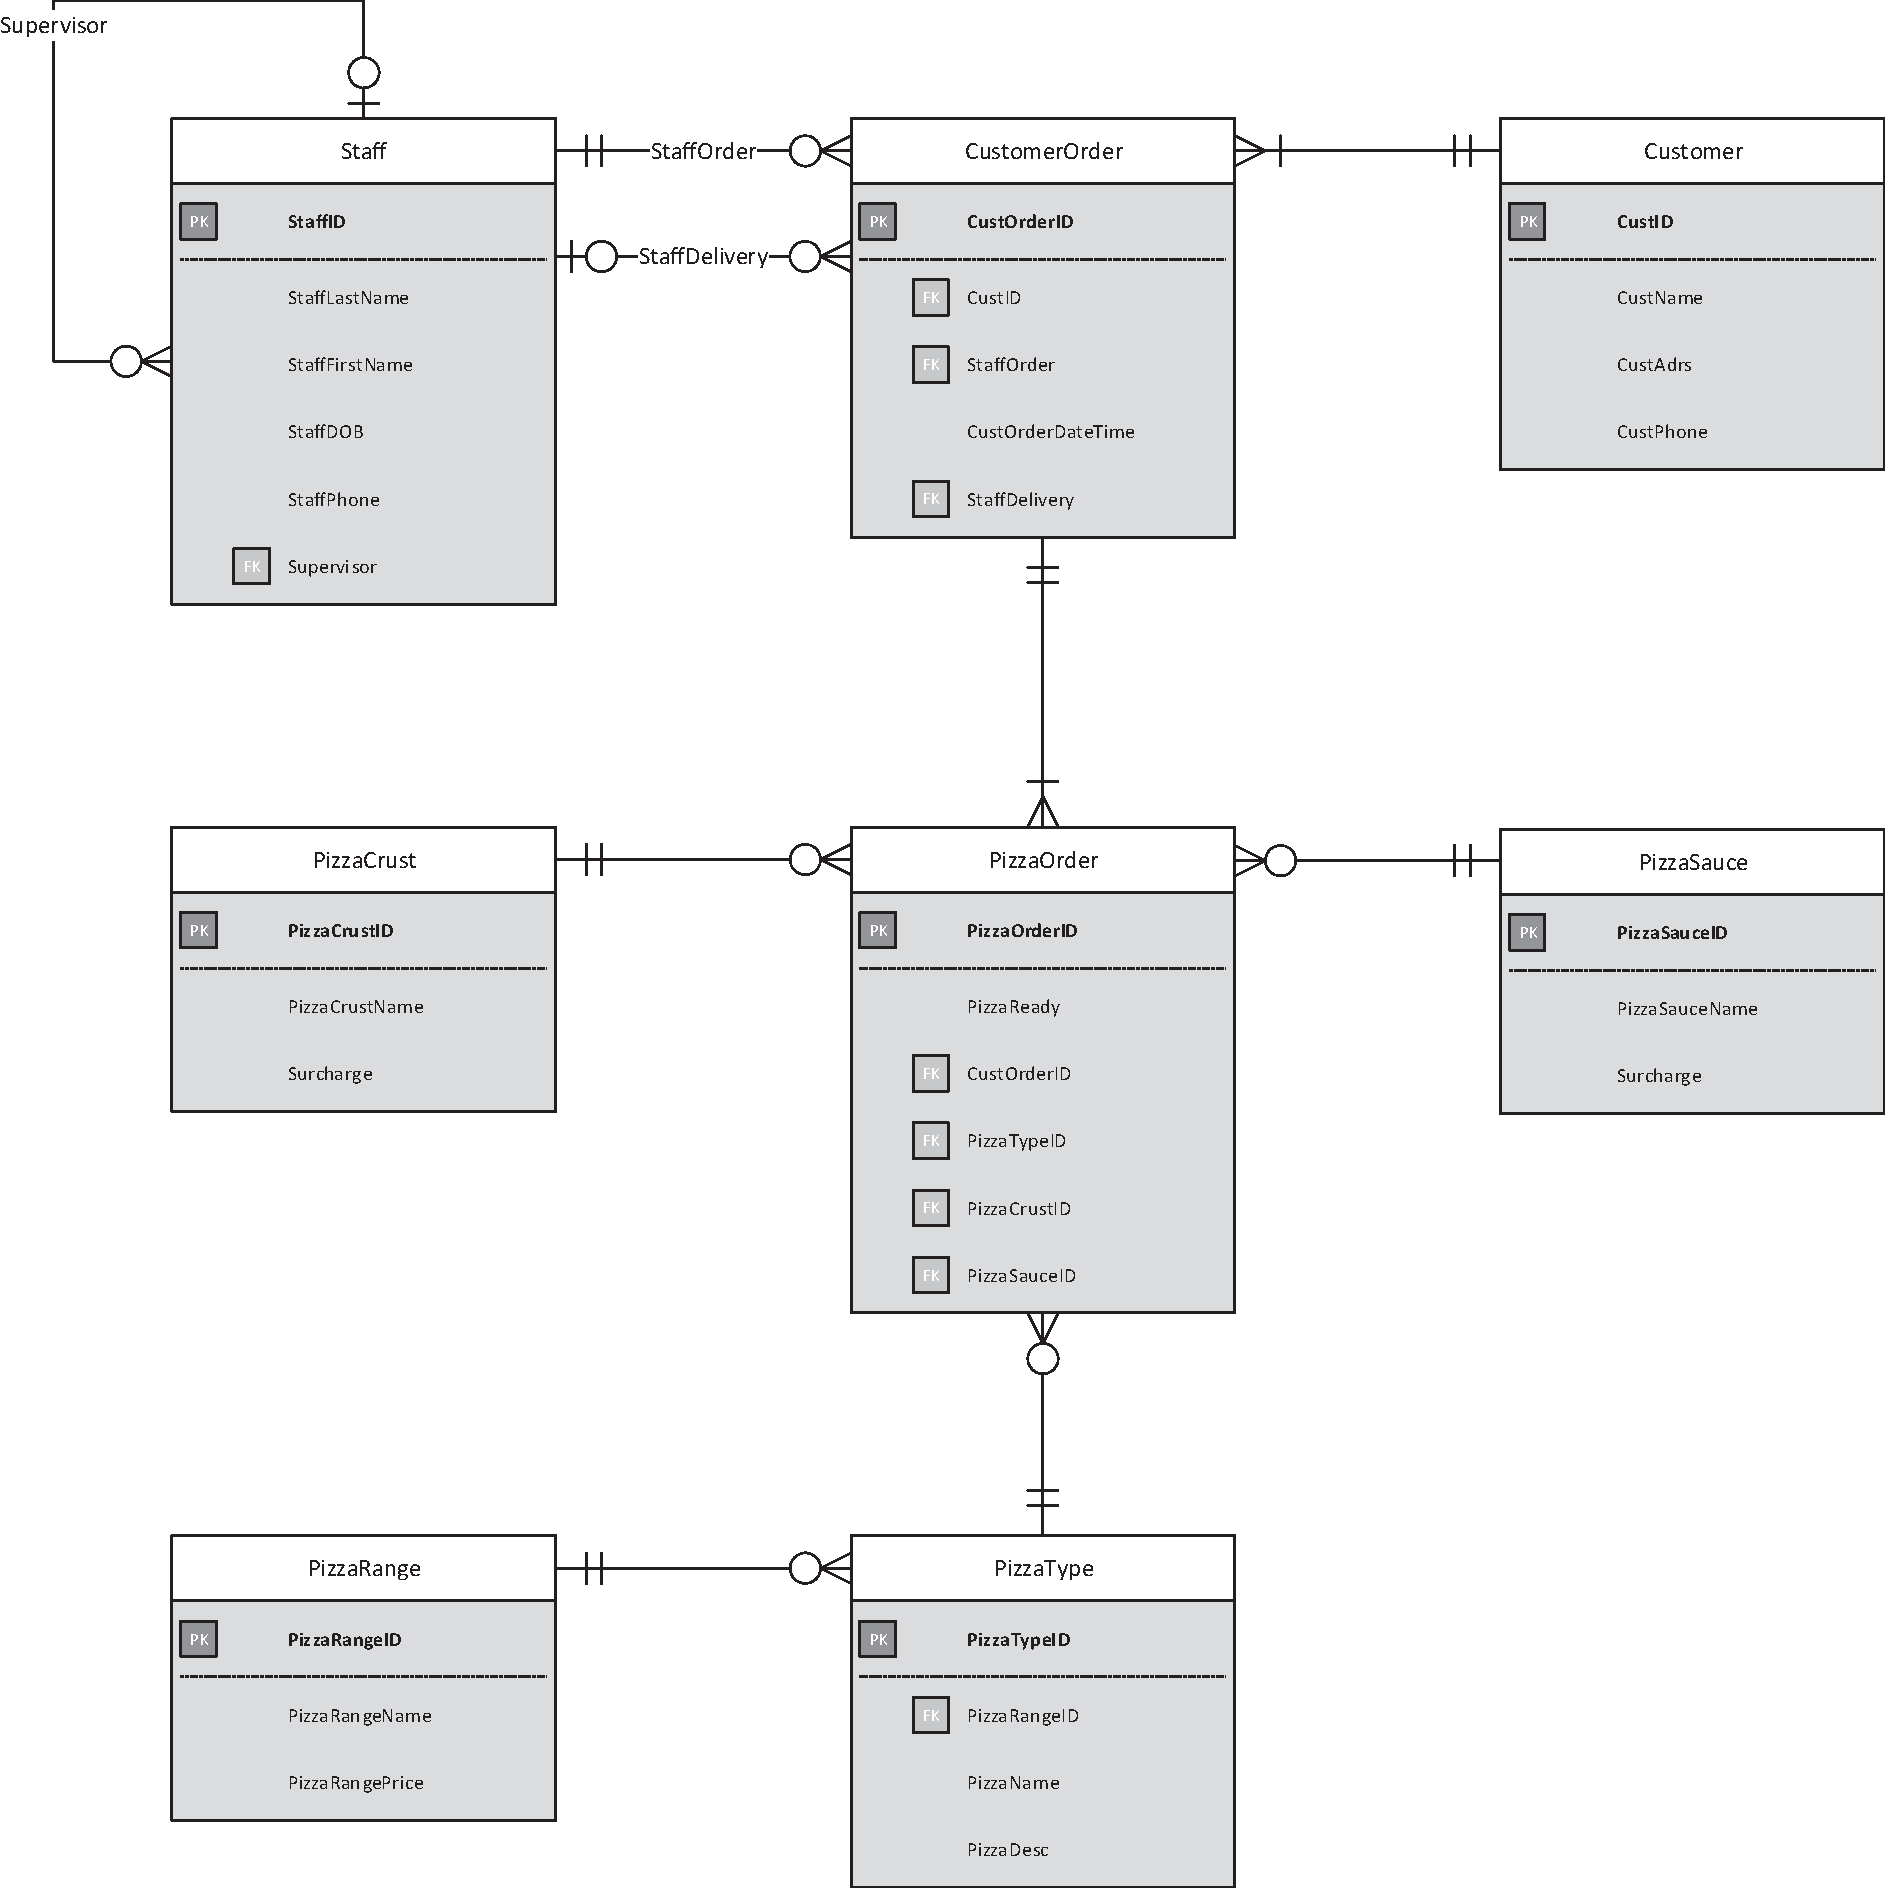
\includegraphics[scale=0.5]{./img/CSG1207_A1_PONCE_TASK_4_ADVPER_PIZZA.pdf}
\end{figure}

\newpage
\subsection{Data Dictionary \& Creation Order}

\begin{table}[H]
  \centering
  \caption{\textbf{``staff''} stores details about staff}
    \begin{tabular}{lllll}
    \textbf{Column name} & \textbf{Type/Length} & \textbf{Null} & \textbf{Constraints} & \textbf{Other} \\
    staff\_id & INT   & NOT NULL & PK    & IDENTITY \\
    staff\_last\_name & VARCHAR(20) & NOT NULL &       &  \\
    staff\_first\_name & VARCHAR(20) & NOT NULL &       &  \\
    staff\_dob & DATE  & NOT NULL &       &  \\
    staff\_phone & VARCHAR(20) & NOT NULL &       &  \\
    supervisor & INT   & NULL & FK (staff.staff\_id) &  \\
    %\bottomrule
    \end{tabular}%
  \label{tab:addlabel}%
\end{table}%

\begin{table}[H]
  \centering
  \caption{\textbf{``customer''} stores details about customer}
    \begin{tabular}{lllll}
    \textbf{Column name} & \textbf{Type/Length} & \textbf{Null} & \textbf{Constraints} & \textbf{Other} \\
    cust\_id & INT   & NOT NULL & PK    & IDENTITY \\
    cust\_name & VARCHAR(50) & NOT NULL &       &  \\
    cust\_adrs & TEXT  & NOT NULL &       &  \\
    cust\_phone & VARCHAR(20) & NOT NULL &       &  \\
    \end{tabular}%
  \label{tab:addlabel}%
\end{table}%

\begin{table}[H]
  \centering
  \caption{\textbf{``customer\_order''} stores details about customer order}
    \begin{tabular}{lllll}
    \textbf{Column name} & \textbf{Type/Length} & \textbf{Null} & \textbf{Constraints} & \textbf{Other} \\
    cust\_order\_id & INT   & NOT NULL & PK    & IDENTITY \\
    cust\_id & INT   & NOT NULL & FK (customer.cust\_id) &  \\
    staff\_order & INT   & NOT NULL & FK (staff.staff\_id) &  \\
    cust\_order\_datetime & DATETIME & NOT NULL &       &  \\
    staff\_delivery & INT   & NULL  & FK (staff.staff\_id) &  \\
    \end{tabular}%
  \label{tab:addlabel}%
\end{table}%

\begin{table}[H]
  \centering
  \caption{\textbf{``pizza\_crust''} stores details about pizza crust}
    \begin{tabular}{lllll}
    \textbf{Column name} & \textbf{Type/Length} & \textbf{Null} & \textbf{Constraints} & \textbf{Other} \\
    pizza\_crust\_id & INT   & NOT NULL & PK    & IDENTITY \\
    pizza\_crust\_name & VARCHAR(20) & NOT NULL &       &  \\
    surcharge & MONEY & NOT NULL &       &  \\
    \end{tabular}%
  \label{tab:addlabel}%
\end{table}%

\begin{table}[H]
  \centering
  \caption{\textbf{``pizza\_sauce''} stores details about pizza sauce}
    \begin{tabular}{lllll}
    \textbf{Column name} & \textbf{Type/Length} & \textbf{Null} & \textbf{Constraints} & \textbf{Other} \\
    pizza\_sauce\_id & INT   & NOT NULL & PK    & IDENTITY \\
    pizza\_sauce\_name & VARCHAR(20) & NOT NULL &       &  \\
    surcharge & MONEY & NOT NULL &       &  \\
    \end{tabular}%
  \label{tab:addlabel}%
\end{table}%

\begin{table}[H]
  \centering
  \caption{\textbf{``pizza\_range''} stores details about pizza range}
    \begin{tabular}{lllll}
    \textbf{Column name} & \textbf{Type/Length} & \textbf{Null} & \textbf{Constraints} & \textbf{Other} \\
    pizza\_range\_id & INT   & NOT NULL & PK    & IDENTITY \\
    pizza\_range\_name & VARCHAR(20) & NOT NULL &       &  \\
    pizza\_range\_price & MONEY & NOT NULL &       &  \\
    \end{tabular}%
  \label{tab:addlabel}%
\end{table}%

\begin{table}[H]
  \centering
  \caption{\textbf{``pizza\_type''} stores details about pizza type}
    \begin{tabular}{lllll}
    \textbf{Column name} & \textbf{Type/Length} & \textbf{Null} & \textbf{Constraints} & \textbf{Other} \\
    pizza\_type\_id & INT   & NOT NULL & PK    & IDENTITY \\
    pizza\_range\_id & INT   & NOT NULL & FK (pizza\_range.pizza\_range\_id) &  \\
    pizza\_name & VARCHAR(20) & NOT NULL &       &  \\
    pizza\_desc & TEXT  & NOT NULL &       &  \\
    \end{tabular}%
  \label{tab:addlabel}%
\end{table}%

\begin{table}[H]
  \centering
  \caption{\textbf{``pizza\_order''} stores details about pizza order}
    \begin{tabular}{lllll}
    \textbf{Column name} & \textbf{Type/Length} & \textbf{Null} & \textbf{Constraints} & \textbf{Other} \\
    pizza\_order\_id & INT   & NOT NULL & PK    & IDENTITY \\
    pizza\_ready & BIT   & NOT NULL &       & DEFAULT 0 \\
    cust\_order\_id & INT   & NOT NULL & FK (customer.cust\_id) &  \\
    pizza\_type\_id & INT   & NOT NULL & FK (pizza\_type.pizza\_type\_id) &  \\
    pizza\_crust\_id & INT   & NOT NULL & FK (pizza\_crust.pizza\_crust\_id) &  \\
    pizza\_sauce\_id & INT   & NOT NULL & FK (pizza\_sauce.pizza\_sauce\_id) &  \\
    \end{tabular}%
  \label{tab:addlabel}%
\end{table}%


